% Soma: CisLunar Rings -- project brief
% Compile with pdfLaTeX (Overleaf default). Figures live in figures/.
\documentclass[11pt,a4paper]{article}

\usepackage[margin=2.2cm]{geometry}
\usepackage[T1]{fontenc}
\usepackage{lmodern}
\usepackage{microtype}
\usepackage{amsmath}
\usepackage{siunitx}
\sisetup{group-separator={,},group-minimum-digits=4}
\usepackage{graphicx}
\usepackage{booktabs}
\usepackage{tabularx}
\usepackage{enumitem}
\usepackage{caption}
\usepackage{float}
\usepackage{xcolor}
\usepackage{fancyhdr}
\usepackage{titlesec}
\usepackage[hidelinks]{hyperref}

\definecolor{somagold}{HTML}{B07A1E}
\definecolor{somateal}{HTML}{2B6F80}
\hypersetup{colorlinks=true,linkcolor=somateal,urlcolor=somateal}

\titleformat{\section}{\large\bfseries\color{somateal}}{\thesection}{0.8em}{}
\captionsetup{font=small,labelfont={bf,color=somateal}}

\pagestyle{fancy}
\fancyhf{}
\fancyhead[L]{\small\color{somateal}Soma: CisLunar Rings}
\fancyhead[R]{\small\color{somateal}Project brief}
\fancyfoot[C]{\small\thepage}
\renewcommand{\headrulewidth}{0.3pt}

\newcommand{\repo}{\href{https://github.com/varunpra97/SomaCislunarSettlement}{github.com/varunpra97/SomaCislunarSettlement}}

\title{\vspace{-1.5em}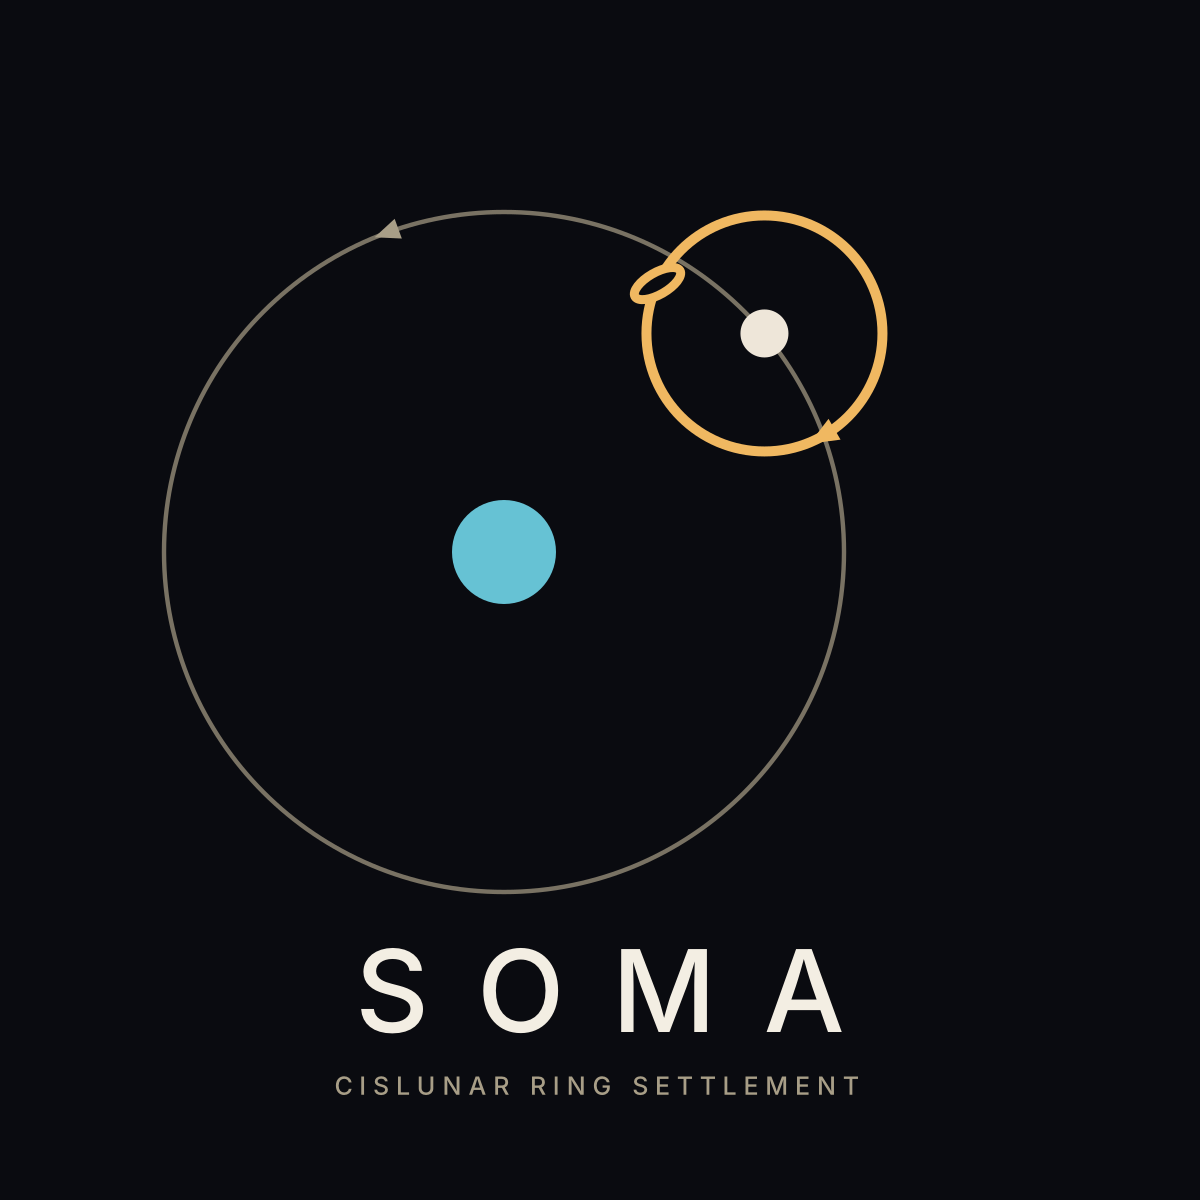
\includegraphics[width=0.32\textwidth]{figures/logo.png}\\[0.6em]
  \textbf{Soma: CisLunar Rings}\\[0.2em]\large A cislunar ring settlement design study}
\author{Varun Prakash}
\date{3 November 2026}

\begin{document}
\maketitle
\thispagestyle{fancy}

\section{Summary}
Soma is a speculative design study for a cislunar ring settlement: six rings, each
\SI{109}{km} around (\SI{34.7}{km} across), on one shared spine, housing about
3.3 million people, parked in a stable loop around the Moon. Each ring is built mostly
from lunar material by self-assembling bay factories, at an estimated
\$87k--661k of build cost per resident. All figures are order-of-magnitude estimates
for a concept, not engineering results.

\begin{figure}[H]
  \centering
  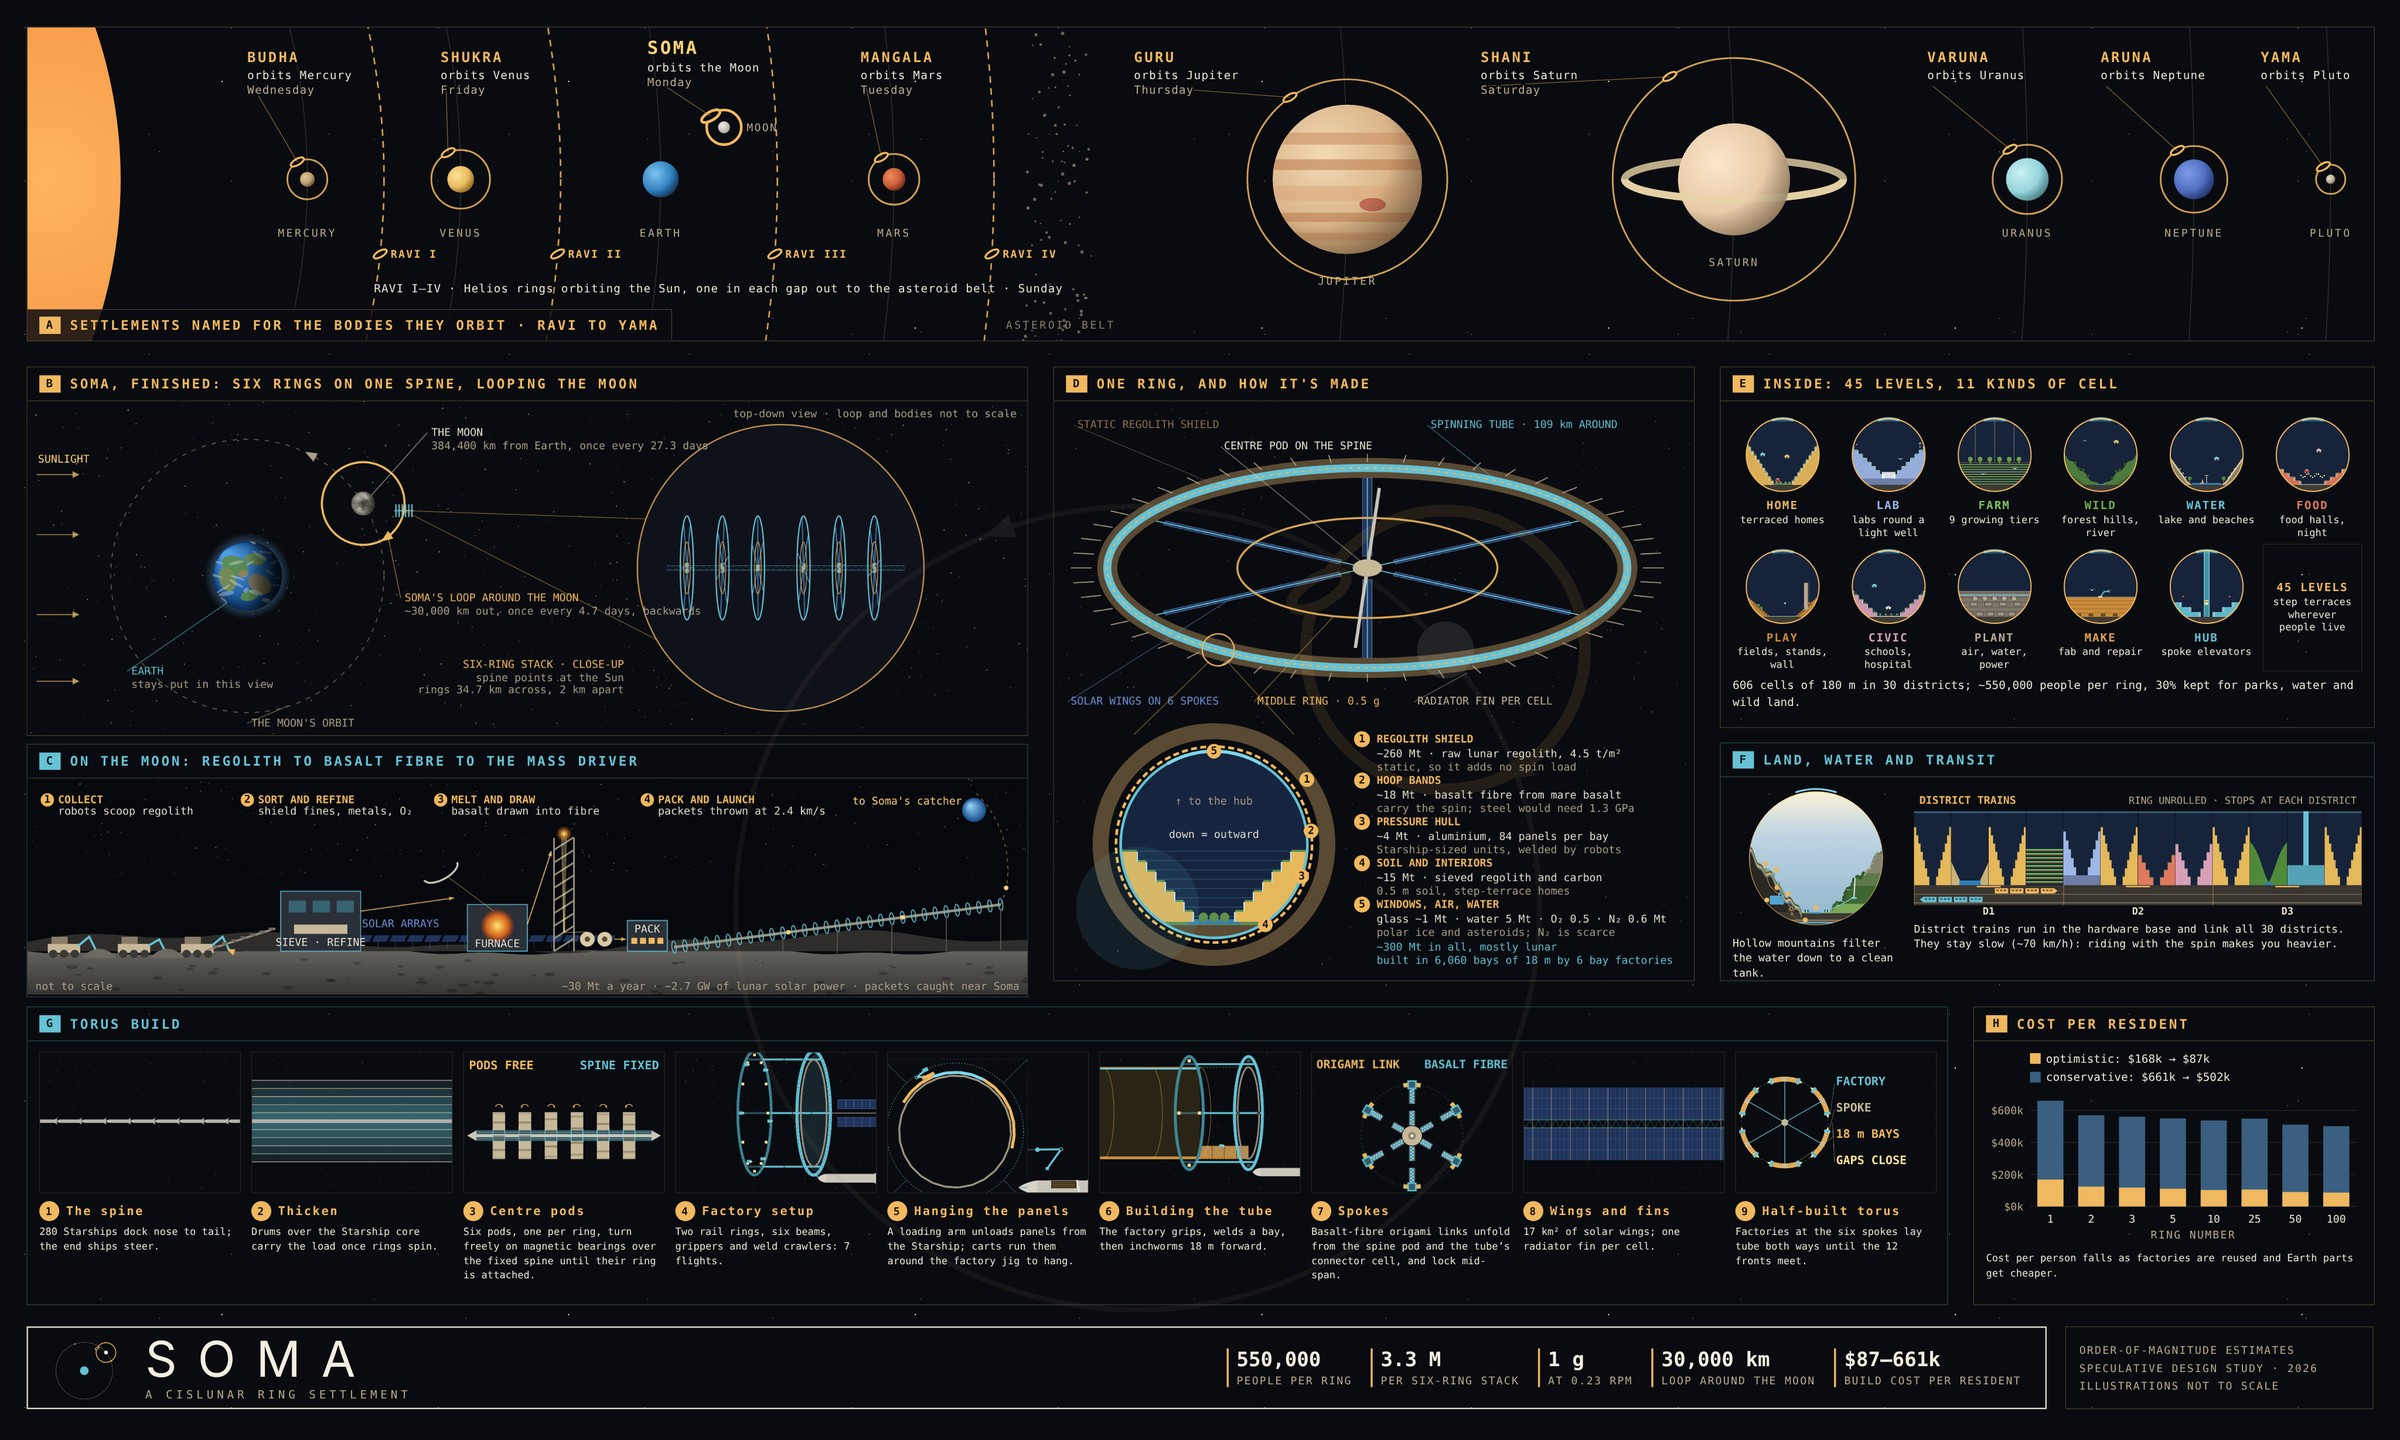
\includegraphics[width=\textwidth]{figures/poster.jpg}
  \caption{The Soma poster ($60 \times 36$\,in). An animated version, in which every
  tile plays its build step, is in the repository.}
\end{figure}

\section{The design}
Each ring is a \SI{150}{m}-wide tube bent into a \SI{17.35}{km}-radius torus that spins
at \SI{0.23}{rpm} for 1\,g at the floor:
\begin{equation}
  a = \omega^2 R, \qquad
  \omega = \sqrt{\frac{9.81\ \mathrm{m\,s^{-2}}}{17\,350\ \mathrm{m}}}
  \approx 0.0238\ \mathrm{rad\,s^{-1}} \approx 0.23\ \mathrm{rpm},
  \qquad v = \omega R \approx 412\ \mathrm{m\,s^{-1}}.
\end{equation}

\begin{figure}[H]
  \centering
  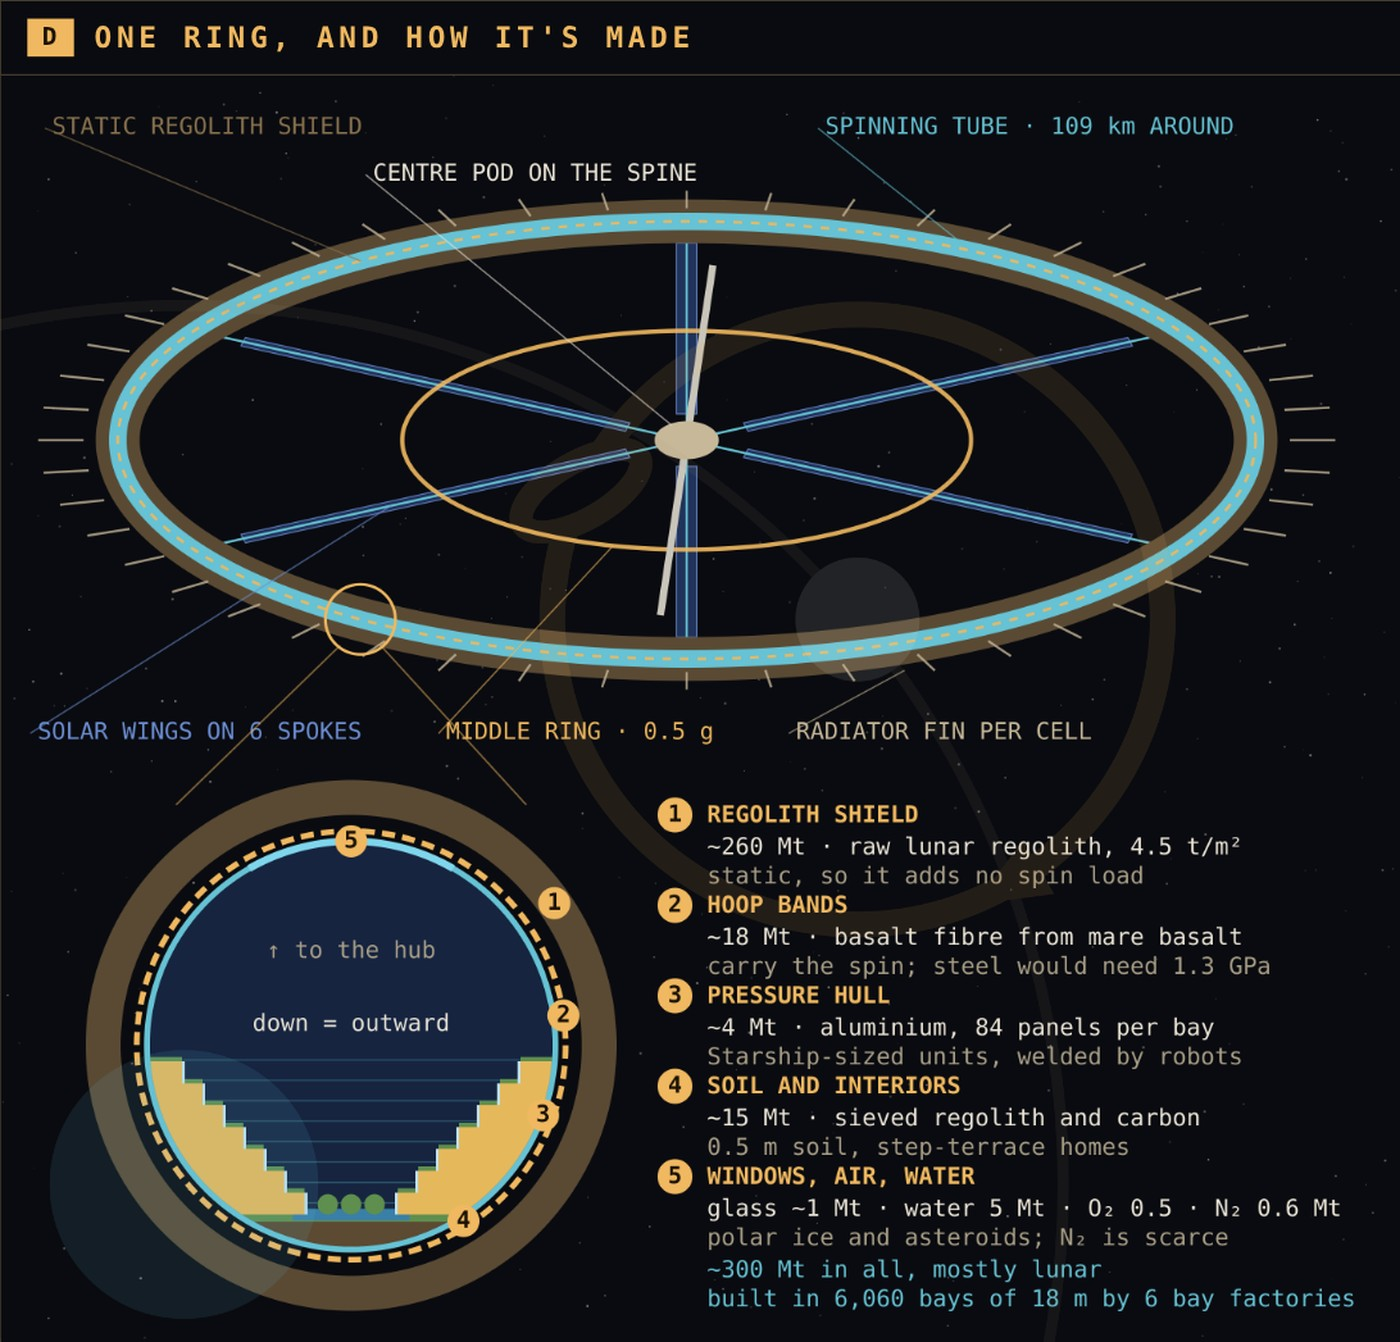
\includegraphics[width=0.62\textwidth]{figures/onering.jpg}
  \caption{One ring and how it is made: shield, hoop bands, hull, soil and terraced interiors.}
\end{figure}

\begin{itemize}[leftmargin=1.2em,itemsep=0.3em]
  \item \textbf{Tube and shield.} Basalt-fibre hoop bands carry the spin. The hoop
  stress from a ring's own mass is $\sigma = \rho v^2$, so steel would need
  \SI{1.3}{GPa} and is too heavy. A static shell of raw regolith ($\sim$\SI{260}{Mt})
  shields against radiation and adds no spin load.
  \item \textbf{Cells.} The tube is split into 606 cells of \SI{180}{m}, grouped into
  30 districts. Each cell has 45 levels of \SI{3.33}{m} and is one of 11 types
  (home, lab, farm, wild, water, food and night, play, civic, plant, make, hub).
  \item \textbf{Step terraces.} Every cell where people live or work steps back from a
  central canyon, so each level has open sky and its own terrace.
  \item \textbf{Spine.} 280 Starships dock nose to tail into a \SI{14}{km} core, later
  wrapped in five concentric drums out to $r = \SI{100}{m}$ ($\sim$\SI{1.4}{Mt}).
  \item \textbf{Centre pods.} Six pods, one per ring, turn on magnetic bearings around
  the fixed spine.
  \item \textbf{Spokes.} Origami-style basalt-fibre links unfold from both the pod and
  the tube's connector cell and lock mid-span. Spin pulls
  $\sigma = \rho v^2/2 \approx \SI{0.23}{GPa}$ on a spoke; basalt fibre holds
  $\sim$\SI{1.5}{GPa}.
  \item \textbf{Stack.} Six rings in three counter-rotating pairs, \SI{2}{km} apart, so
  the stack has no net spin and can be steered like a gyroscope to face the Sun.
  \item \textbf{Power and heat.} Solar wings on the six spokes ($\sim$\SI{6}{GW}) face
  the Sun at all times because the spin axis points at it. About 650 radiator fins,
  one per cell, shed heat edge-on.
  \item \textbf{Transit.} District trains run through the hardware base at
  $\sim$\SI{70}{km/h}. They stay slow because riding with the spin makes you feel heavier.
\end{itemize}

\begin{figure}[H]
  \centering
  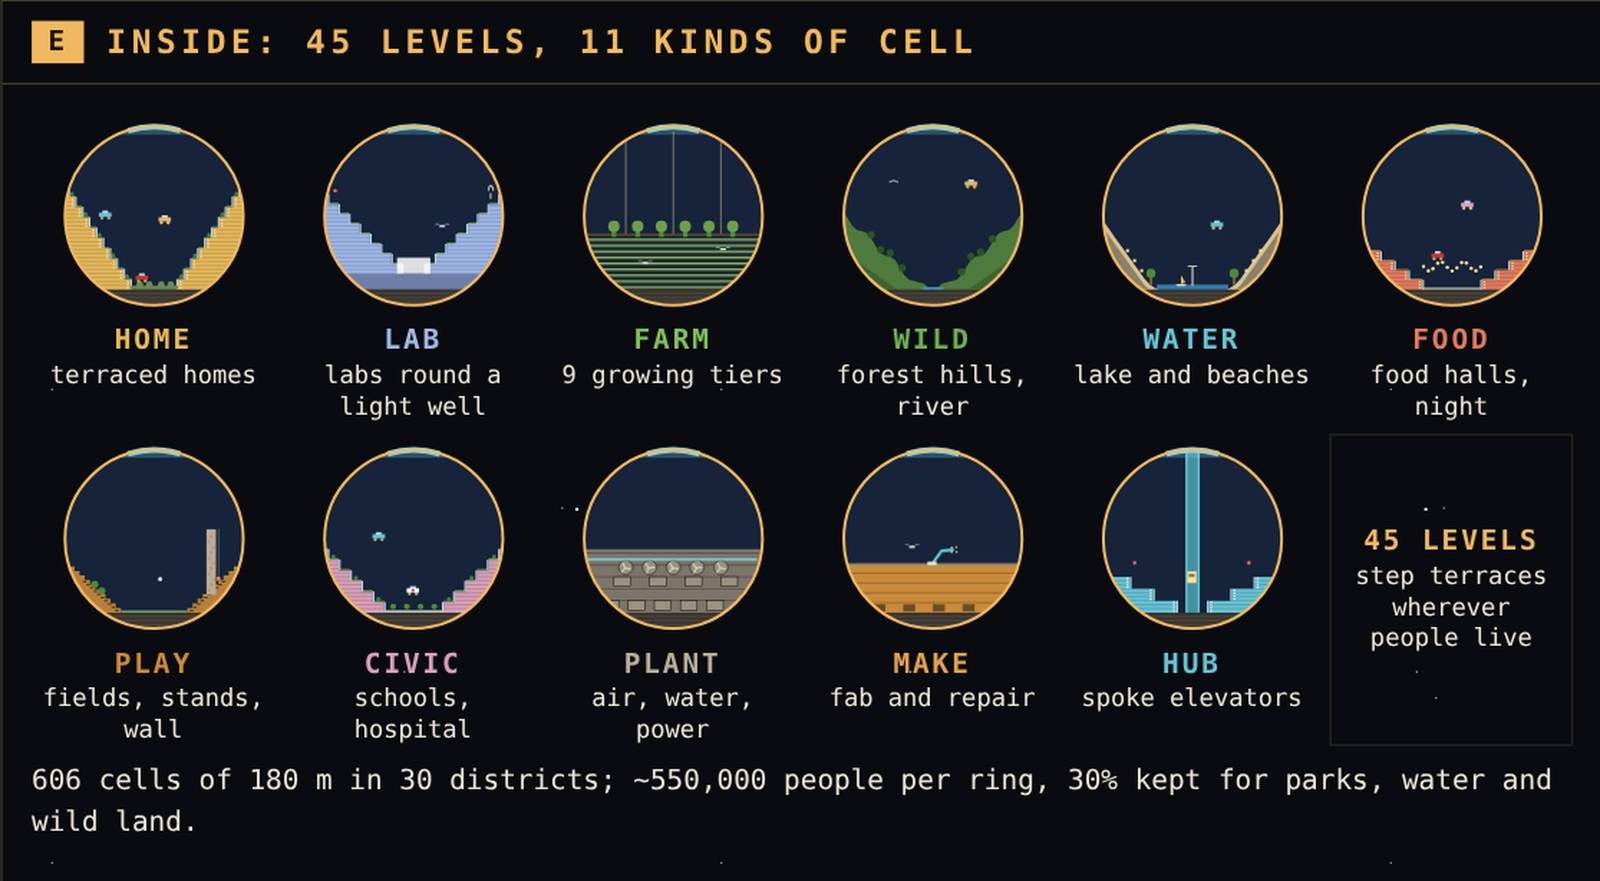
\includegraphics[width=0.85\textwidth]{figures/cells.jpg}
  \caption{The 11 cell types in cross-section, with step terraces wherever people live.}
\end{figure}

\begin{figure}[H]
  \centering
  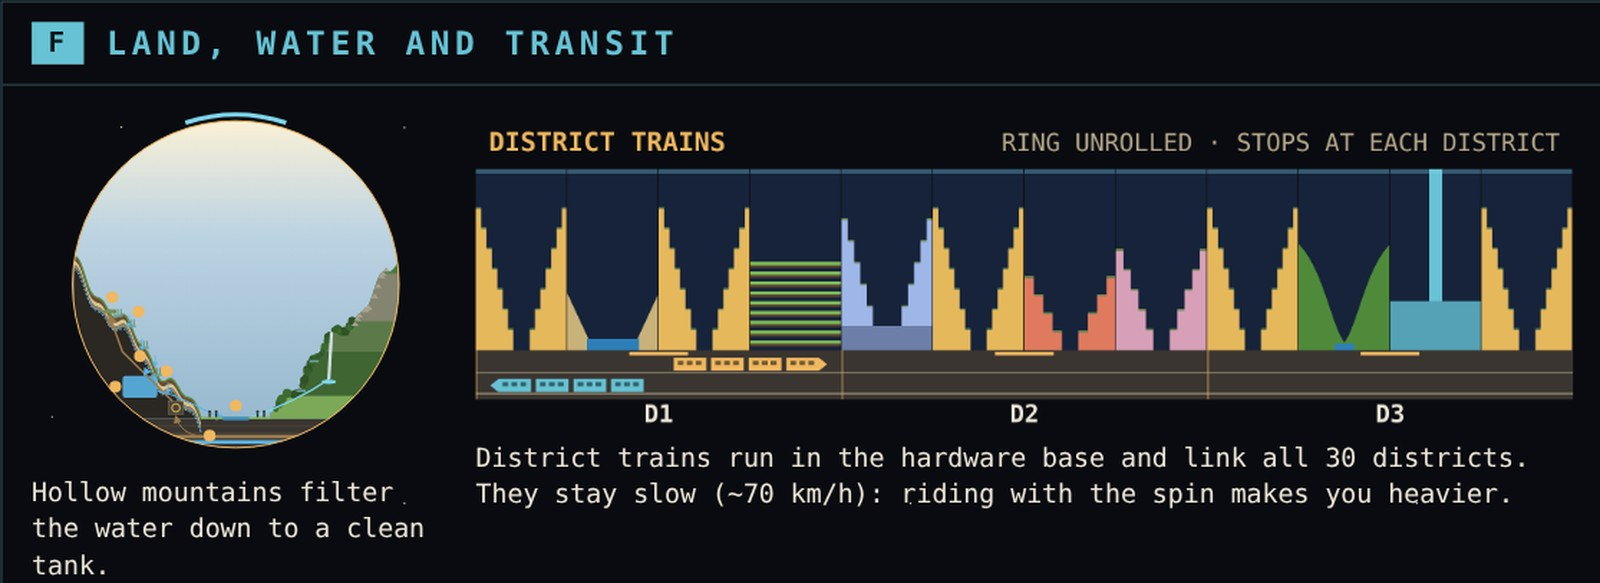
\includegraphics[width=0.85\textwidth]{figures/transit.jpg}
  \caption{Land, water and transit: a filter mountain and district trains in the hardware base.}
\end{figure}

\section{How it is built}
The build runs in nine steps, starting from the spine and ending when the tube closes
into a ring. The full construction film, \emph{How Soma is built} (5\,min\,57\,s), is
in the repository under
\nolinkurl{videos/soma-construction-film.mp4}.

\begin{enumerate}[leftmargin=1.5em,itemsep=0.3em]
  \item \textbf{The spine.} Cargo Starships unload, then dock nose to tail along the
  spin axis; the ships at each end keep their engines to steer.
  \item \textbf{Thicken.} Concentric drums are wrapped over the Starship core so it can
  carry Sun-tracking loads once the rings spin.
  \item \textbf{Centre pods.} Six pods are built over the fixed spine one by one. They
  turn freely on magnetic bearings; real spin waits until the ring is attached.
  \item \textbf{Factory setup.} Seven Starship flights bring two rail rings, six beams,
  grippers and weld crawlers for each bay factory.
  \item \textbf{Hanging the panels.} A loading arm unloads hull panels from a Starship;
  carts run them around the factory jig to hang.
  \item \textbf{Building the tube.} The factory grips the tube, welds and leak-tests one
  \SI{18}{m} bay, then inchworms forward.
  \item \textbf{Spokes.} Origami links unfold from the pod and the tube's connector cell
  and lock mid-span, in balanced pairs.
  \item \textbf{Wings and fins.} Wing robots unroll \SI{17}{km^2} of lunar-made solar
  cells along the spokes; carriers fit one radiator fin per cell.
  \item \textbf{Half-built torus to full ring.} Six factories build tube both ways from
  the spokes; the 12 fronts meet after 6,060 bays and the ring closes.
\end{enumerate}

\begin{figure}[H]
  \centering
  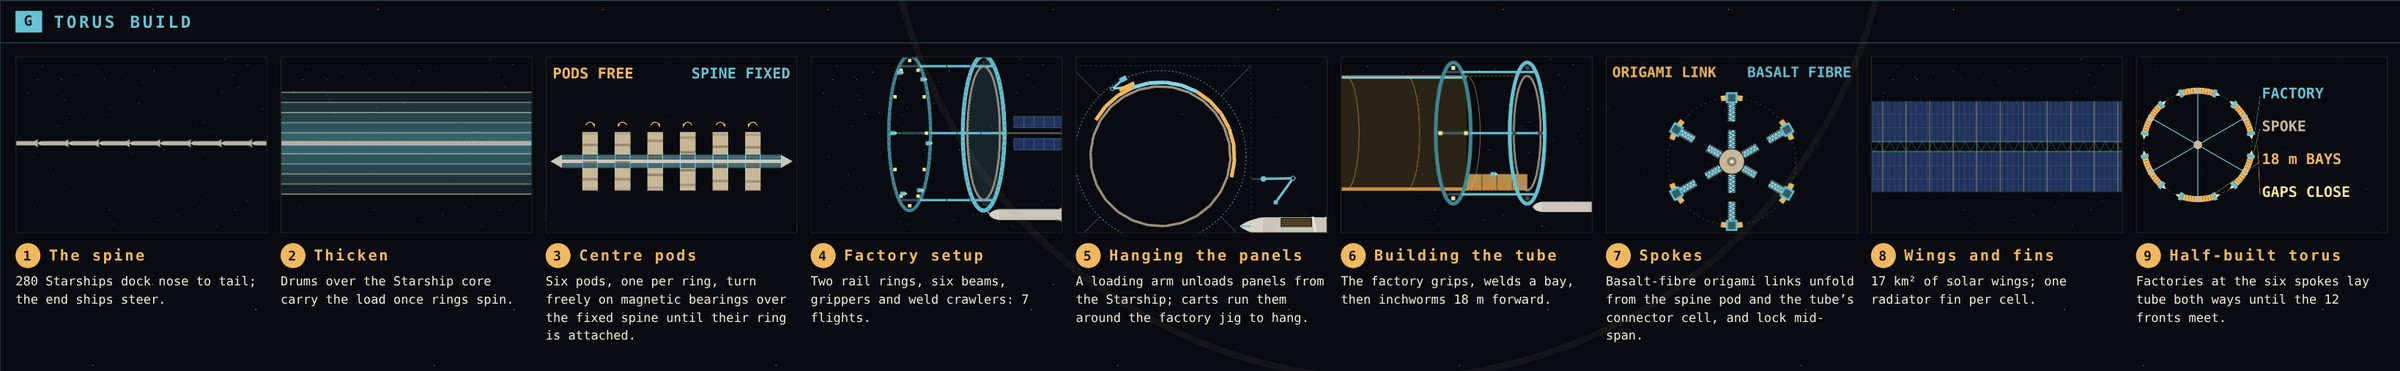
\includegraphics[width=\textwidth]{figures/build.jpg}
  \caption{The nine build steps, from the spine to the half-built torus.}
\end{figure}

On the Moon, robots collect regolith, plants sort it and draw basalt into fibre, and a
mass driver throws packets at \SI{2.4}{km/s} to a catcher near Soma
($\sim$\SI{30}{Mt} a year).

\begin{figure}[H]
  \centering
  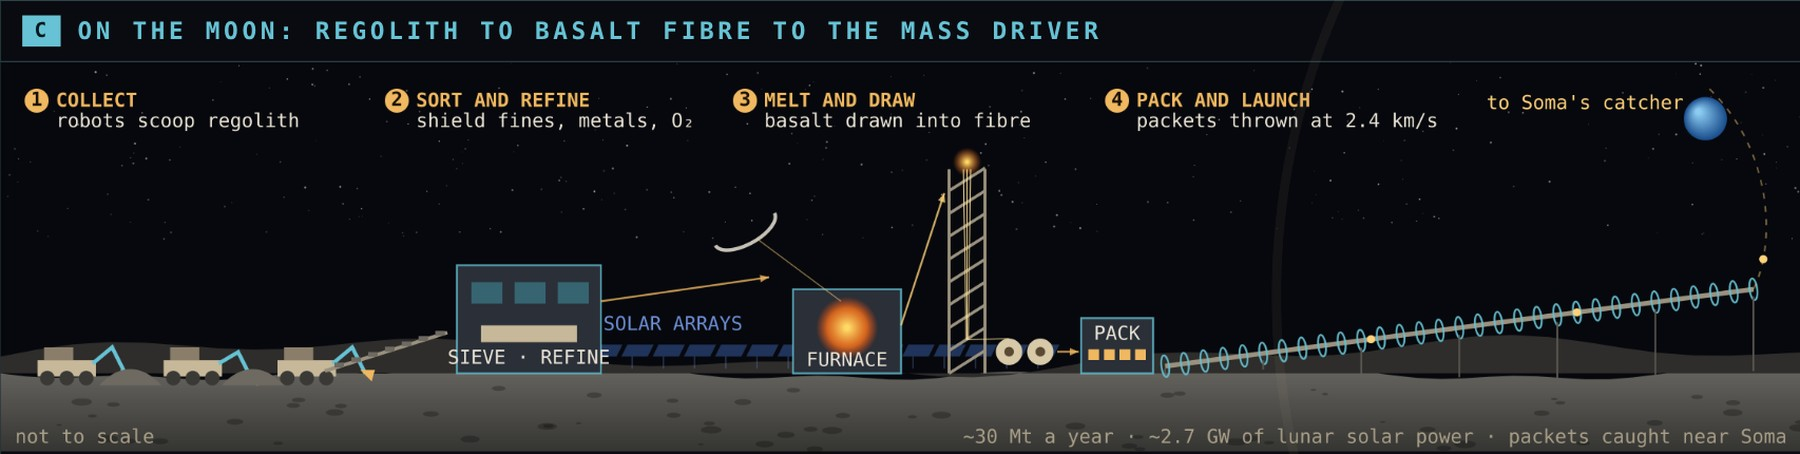
\includegraphics[width=\textwidth]{figures/lunar.jpg}
  \caption{On the Moon: regolith to basalt fibre to the mass driver.}
\end{figure}

\section{Orbit}
Soma sits in a lunar distant retrograde orbit about \SI{30000}{km} from the Moon,
looping it backwards every 4.7 days while the Moon carries it around Earth. In a
simplified Earth--Moon--Sun model it stayed bound for 20 years with no corrections,
even with a \SI{2}{m/s} kick each time a ring was added. Larger loops
(40,000--70,000\,km) drifted off within 2--4 years. The Soma logo is drawn from this orbit.

\begin{figure}[H]
  \centering
  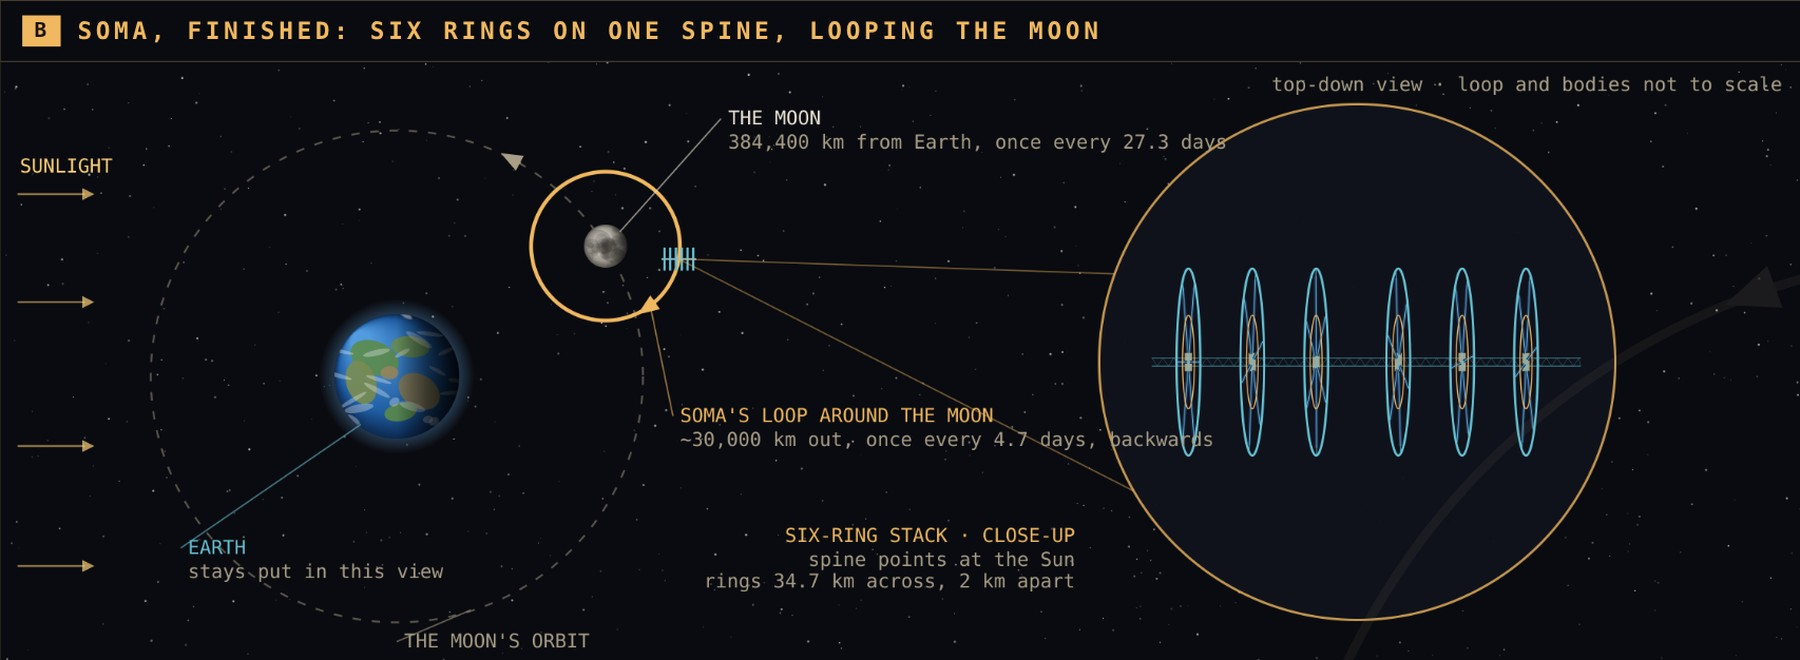
\includegraphics[width=\textwidth]{figures/orbit.jpg}
  \caption{Soma's loop around the Moon, top-down with Earth fixed.}
\end{figure}

\section{Cost per resident}
Build cost per resident falls from \$168k--661k for ring 1 to \$87k--502k for ring 100,
because later rings reuse the lunar industry and factories and Earth-made parts get
cheaper. The range runs from an optimistic case (80\% learning curve) to a conservative
one (90\%). A standalone ring costs about \$89--356B; 100 rings total about \$5.2T
(optimistic) to \$28.7T (conservative).

\section{Key numbers}
\begin{table}[H]
  \centering
  \begin{tabularx}{\textwidth}{@{}lX@{}}
    \toprule
    \textbf{Item} & \textbf{Value} \\
    \midrule
    Ring & \SI{109}{km} around, \SI{17.35}{km} radius, 1\,g at \SI{0.23}{rpm} \\
    Tube & \SI{150}{m} across, 45 levels of \SI{3.33}{m}, 606 cells of \SI{180}{m} \\
    Population & $\sim$550,000 per ring; $\sim$3.3 million per six-ring stack \\
    Atmosphere & \SI{57}{kPa}, 34\% O$_2$ \\
    Mass per ring & $\sim$\SI{300}{Mt}, mostly lunar regolith \\
    Spine & 280 Starships (\SI{14}{km} core) + 5 drums to $r = \SI{100}{m}$, $\sim$\SI{1.4}{Mt} \\
    Middle ring & $r = \SI{8.7}{km}$, 0.5\,g, \O\ \SI{40}{m} \\
    Stack & 6 rings, 3 counter-rotating pairs, \SI{2}{km} apart \\
    Power & $\sim$\SI{6}{GW} per ring from spoke wings \\
    Orbit & Lunar DRO, $\sim$\SI{30000}{km}, 4.7-day loop \\
    Cost per resident & Ring 1: \$168k--661k $\rightarrow$ ring 100: \$87k--502k \\
    \bottomrule
  \end{tabularx}
\end{table}

\section{Deliverables}
\begin{itemize}[leftmargin=1.2em,itemsep=0.3em]
  \item \textbf{Repository:} \repo, with the README, videos, design boards, logo and
  render scripts.
  \item \textbf{Full report:} \href{https://claude.ai/artifact/T8Bgr5gNkfa1cog84XKW5Q}{Soma: Cost, Deployment and Operations}, 36 pages.
  \item \textbf{Construction film:} \emph{How Soma is built}, 5\,min\,57\,s, from the
  spine to the zoom out to the orbit.
  \item \textbf{Poster:} $60 \times 36$\,in print PDF, plus a 4096\,px image for X.
  \item \textbf{Animated poster:} 8-second looping GIF in which every tile plays its
  build step, at 3840\,px and 1920\,px.
\end{itemize}

\section{Caveats and open questions}
These are concept estimates; the items below would need real engineering before any of
the numbers hold.
\begin{itemize}[leftmargin=1.2em,itemsep=0.2em,label=\fbox{\phantom{\scriptsize x}}]
  \item Basalt-fibre strength and creep at \SI{1.5}{GPa} over decades of spin
  \item How the origami spoke links fold, lock and carry load at \SI{17}{km} length
  \item Long-term orbit stability with a full-physics model, not the planar
  bicircular one used here
  \item Nitrogen supply: lunar N$_2$ is scarce, so it must come from asteroids or Earth
  \item Mass-driver catch accuracy and throughput at $\sim$\SI{30}{Mt} a year
  \item Cost model assumptions: learning rates, Starship launch prices and lunar
  industry ramp
\end{itemize}

\end{document}
